% Section content template for individual Educative lessons
% This file contains the actual content for a specific section
% Generated from Educative API section content

% Section: Class Diagram
% Section ID: 5678758717816832
% Section Slug: class-diagram
% Generated: 2025-12-08T22:21:54.485736

\textbf{Class diagrams} are used to depict the system\textquotesingle s static perspective. They are used in the design process to show the shared roles and responsibilities of the entities that produce the behavior of the system.
\\
Class diagrams are widely used in the modeling of object-oriented designs because this is the only UML diagram that can be directly transferred to object-oriented programming languages.

\subsection{Why use class diagrams?}\label{why-use-class-diagrams}
\\
The following are some important purposes of the class diagram:

\begin{itemize}
\item
Represents the system\textquotesingle s static structure.
\item
Directly maps with object-oriented languages.
\item
Represents what the system\textquotesingle s duties or responsibilities are.
\item
Uses in both forward and reverse engineering.
\end{itemize}

\subsection{Popular notations in the class diagram}\label{popular-notations-in-the-class-diagram}
\\
The following are some essential notations of the class diagram:

\begin{itemize}
\item
Class notation
\item
Interface, abstract class, and enumeration
\item
Access modifiers
\end{itemize}

\subsubsection{Class notation}\label{class-notation}
\\
A class is represented by a rectangle with three sections. The first section holds the class \textbf{name}, the second one lists the \textbf{attributes}, and the third one shows the \textbf{methods} (operations). The following is the depiction of a `\textbf{Movie`} class with its attributes and methods.

\begin{figure}[htbp]
 \centering
 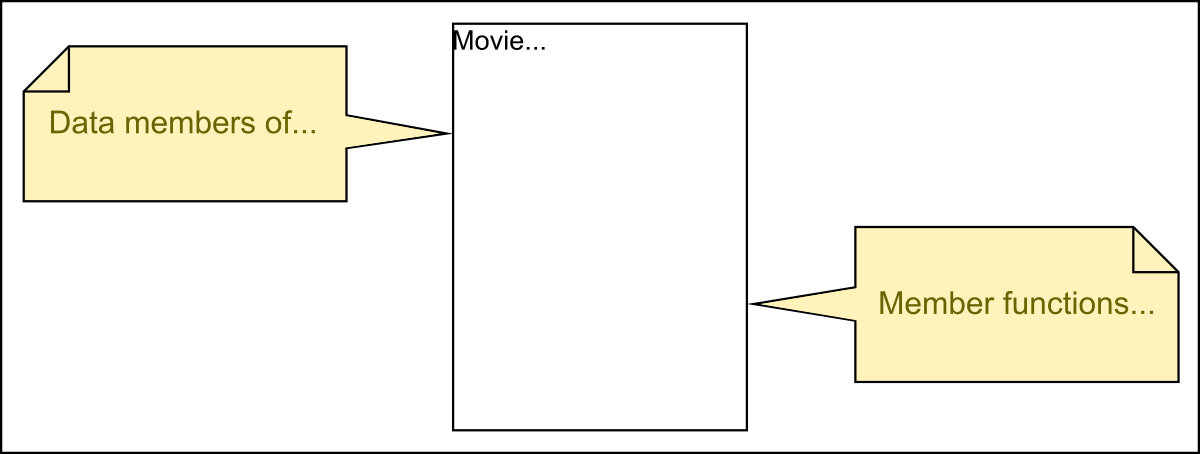
\includegraphics[width=0.5\textwidth]{Images/chapter_3/section_5678758717816832/5293314196897792.png}
 \caption{Notation of a class in a class diagram}
\end{figure}

\subsubsection{Interface, abstract class, and enumeration}\label{interface-abstract-class-and-enumeration}
\\
We can declare a class as abstract using \textbf{abstract} keywords. The class name will be printed in italic. We can use the interface, annotation, and enum keywords too. The illustration below shows how to depict these notations in a class diagram.

\begin{figure}[htbp]
 \centering
 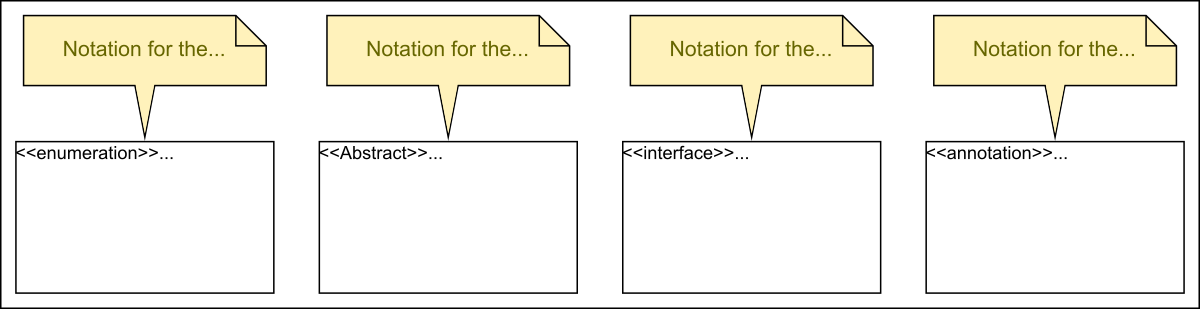
\includegraphics[width=0.5\textwidth]{Images/chapter_3/section_5678758717816832/5850423089692672.png}
 \caption{Class diagram notation for abstract classes, interfaces, enumerations, and annotations}
\end{figure}

\subsubsection{Access modifiers}\label{access-modifiers}
\\
You may use character symbols to specify the visibility of the associated object when defining methods or attributes. The most widely used access modifiers are as follows:
\\
\textbf{Public:} A public member can be seen anywhere in the system. It is represented by a \texttt{+} symbol.
\\
\textbf{Private:} Members can only be accessible from within the class. It is inaccessible from outside the class. It is represented by a \texttt{-} symbol.
\\
\textbf{Protected}: Members are only accessible within the class and derived classes. It is represented by the \# symbol.
\\
The following images show how to use the access modifiers in the class diagram:

\begin{figure}[htbp]
 \centering
 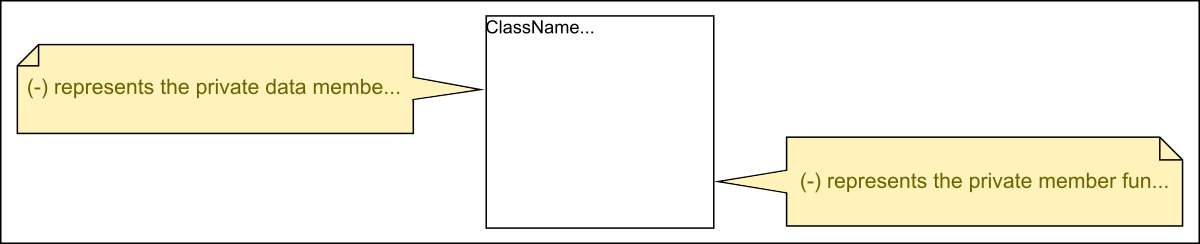
\includegraphics[width=0.5\textwidth]{Images/chapter_3/section_5678758717816832/6025968978493440.png}
 \caption{Access modifiers notations}
\end{figure}

\subsection{Association}\label{association}
\\
\textbf{Association} provides a mechanism to communicate one object with another object, or one object provides services to another object. Association represents the relationship between classes.
\\
The association can be divided into two categories:

\begin{itemize}
\item
Class association (Inheritance)
\item
Object association
\end{itemize}

\begin{center}
\fbox{\begin{minipage}{0.9\textwidth}
\centering
\vspace{0.2cm}
\textit{[Interactive Mind Map - See online version for interactive visualization]}
\vspace{0.2cm}
\end{minipage}}
\end{center}

\vspace{0.3cm}
\begin{itemize}
\item \textbf{Association}
\begin{itemize}
\item \textbf{Class Association}
\begin{itemize}
\item \textbf{Inheritance}
\begin{itemize}
\item \textbf{Single level inheritance}
\end{itemize}
\begin{itemize}
\item \textbf{Multi level inheritance}
\end{itemize}
\begin{itemize}
\item \textbf{Hierarchical inheritance}
\end{itemize}
\begin{itemize}
\item \textbf{Multiple inheritance}
\end{itemize}
\begin{itemize}
\item \textbf{Hybrid inheritance}
\end{itemize}
\end{itemize}
\end{itemize}
\begin{itemize}
\item \textbf{Object Association}
\begin{itemize}
\item \textbf{Simple Association}
\end{itemize}
\begin{itemize}
\item \textbf{Composition}
\end{itemize}
\begin{itemize}
\item \textbf{Aggregation}
\end{itemize}
\end{itemize}
\end{itemize}

\subsubsection{Class association}\label{class-association}
\\
\textbf{Inheritance} falls under the category of class association. Creating a new class from the existing class(es) is called \textbf{inheritance}. Apart from its own behaviors and attributes, the child class inherits the characteristics of its parent(s). A solid line leads from the child class to the parent class with a hollow arrowhead representing the inheritance relationship.
\\
The following class diagram represents the inheritance relationship:

\begin{figure}[htbp]
 \centering
 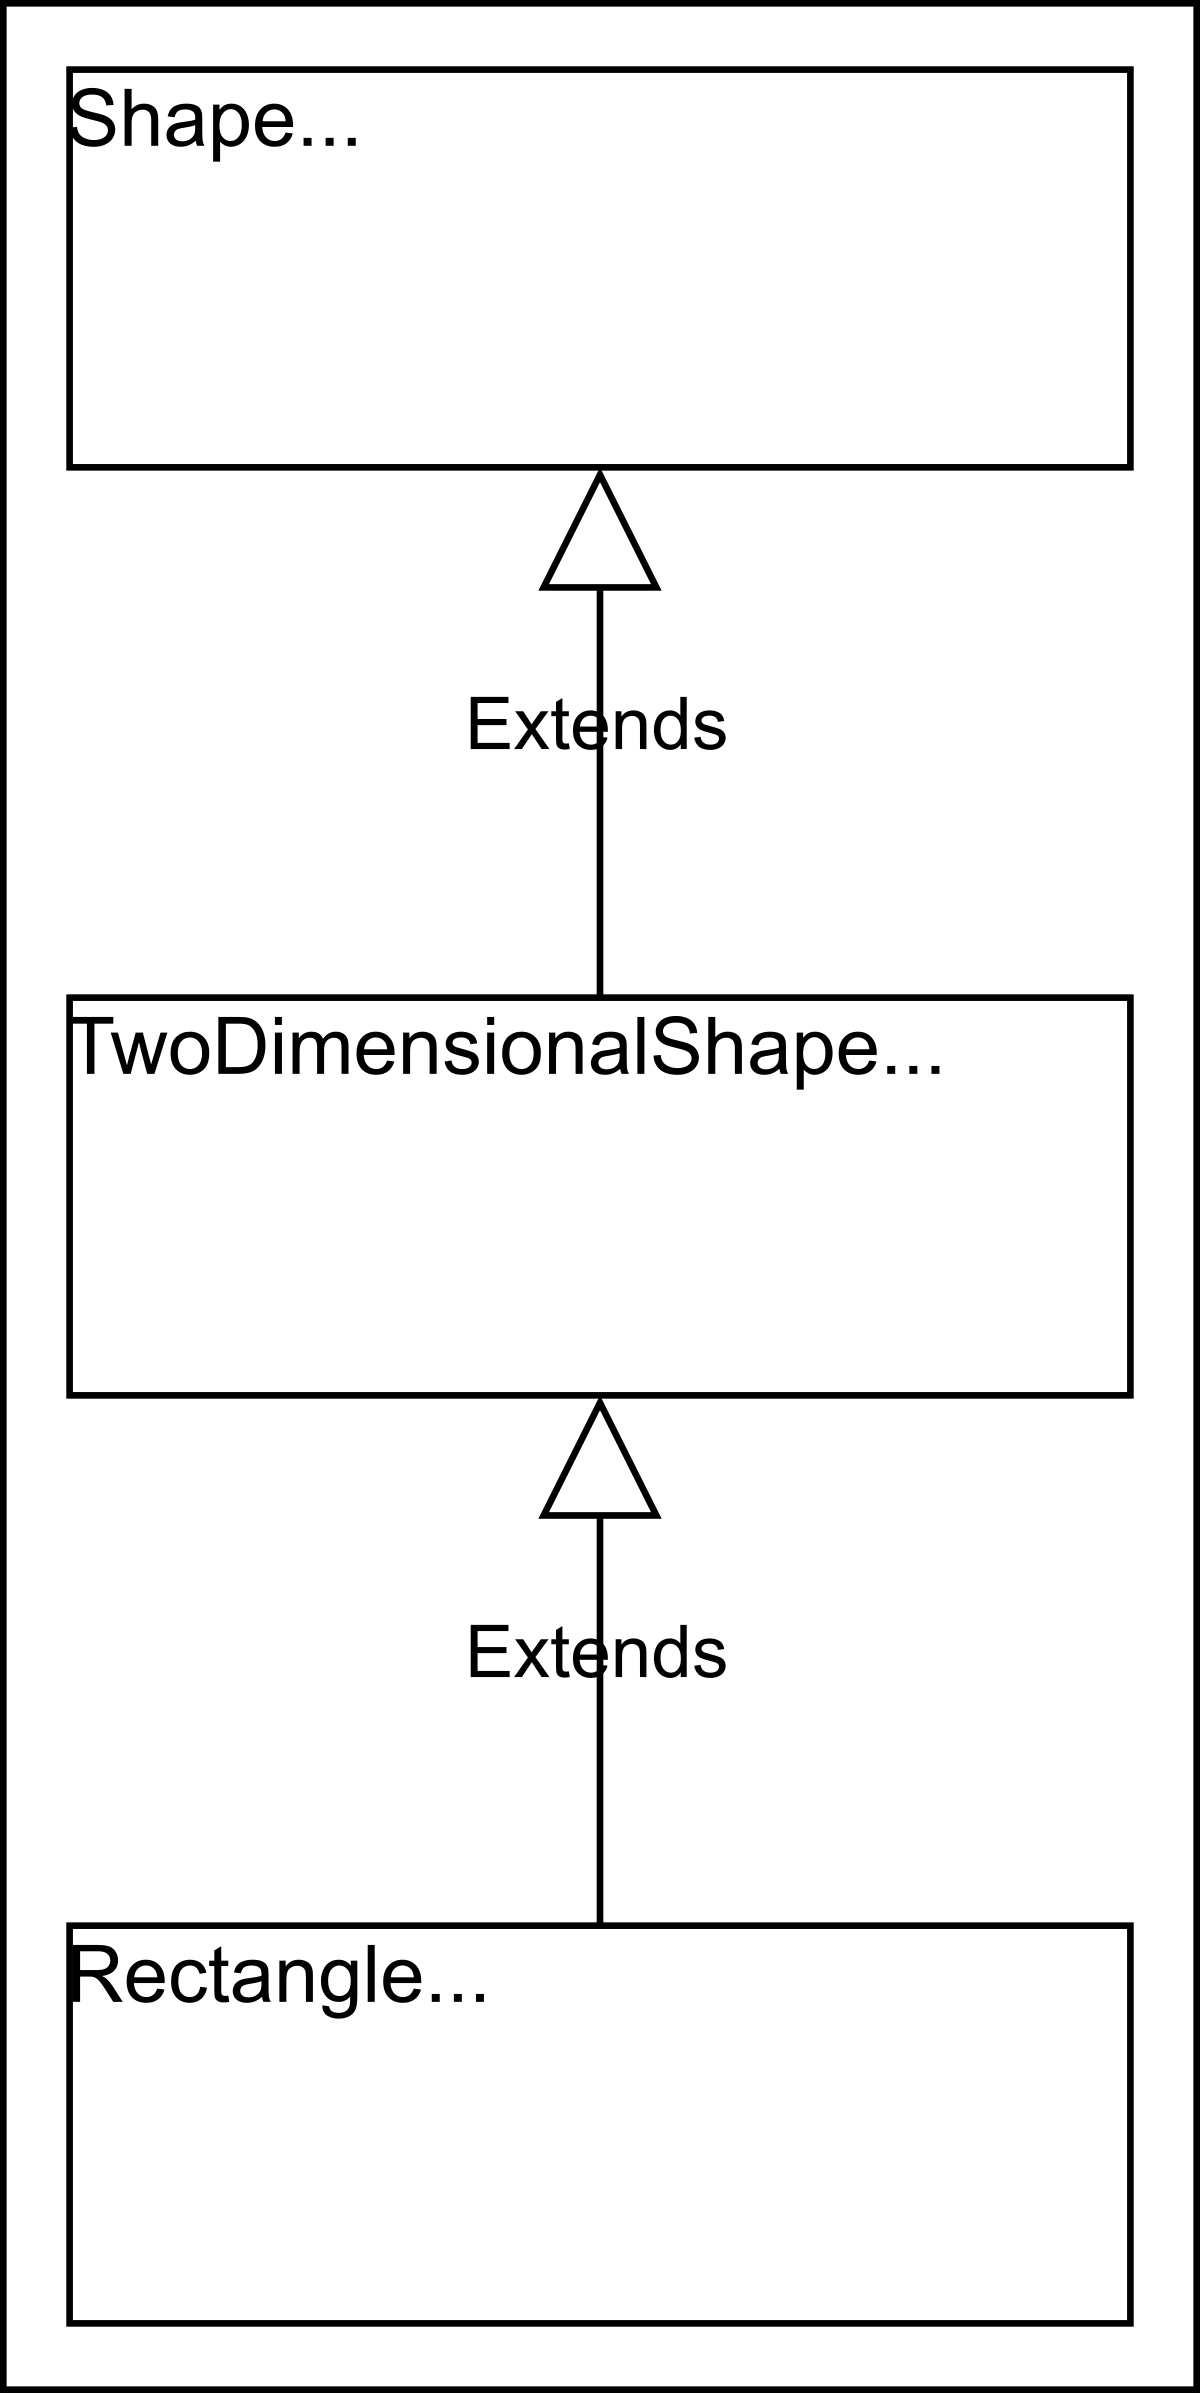
\includegraphics[width=0.25\textwidth]{Images/chapter_3/section_5678758717816832/5303308736790528.png}
 \caption{Class diagram to represent the multi-level inheritance}
\end{figure}

\begin{quote}
\textbf{Note:} We already discussed the different types of inheritance in the \href{https://www.educative.io/courses/grokking-the-low-level-design-interview-using-ood-principles/inheritance}{previous chapter}.
\end{quote}
\subsubsection{Object association}\label{object-association}
\\
Object association (relationship between objects) can be divided into the following categories:
\\
  1. Simple association
\\
  2. Composition
\\
  3. Aggregation
\\
\paragraph{Simple association}\label{simple-association}
\\
The weakest connections between objects are made through \textbf{simple association}. It is achieved through reference, which one object can inherit from another. The following is an example of a simple association:

\begin{figure}[htbp]
 \centering
 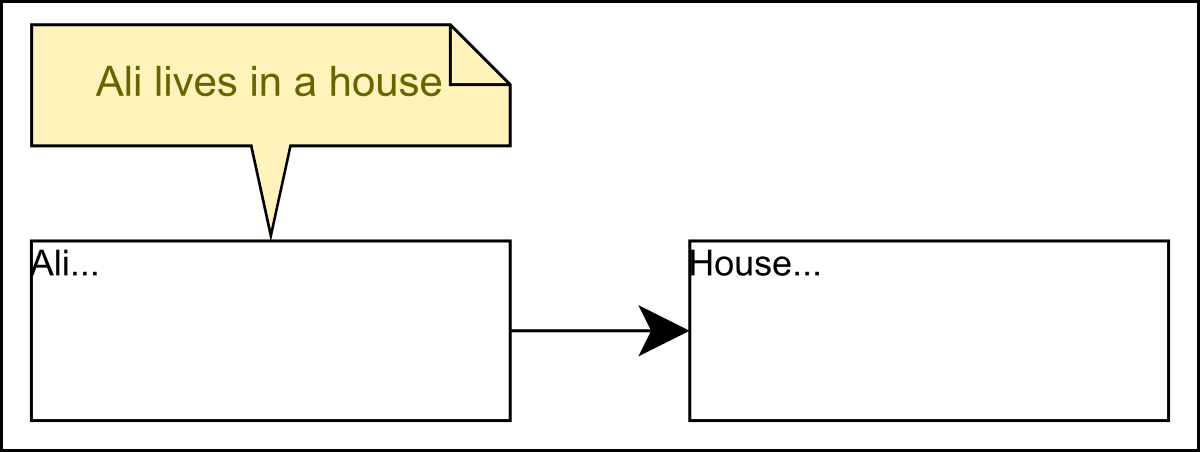
\includegraphics[width=0.5\textwidth]{Images/chapter_3/section_5678758717816832/6353249110327296.png}
 \caption{The class diagram representing a simple association}
\end{figure}

\paragraph{Aggregation}\label{aggregation}
\\
\textbf{Aggregation} describes the relationship between the container and the object it contains. An object may contain an aggregate of another object. Aggregation is denoted by a line with an unfilled diamond head towards the container.
\\
Aggregation is a \emph{weaker} relationship because:

\begin{itemize}
\item
Aggregate objects are not a part of the container.
\item
Aggregate objects can exist independently.
\end{itemize}

\begin{figure}[htbp]
 \centering
 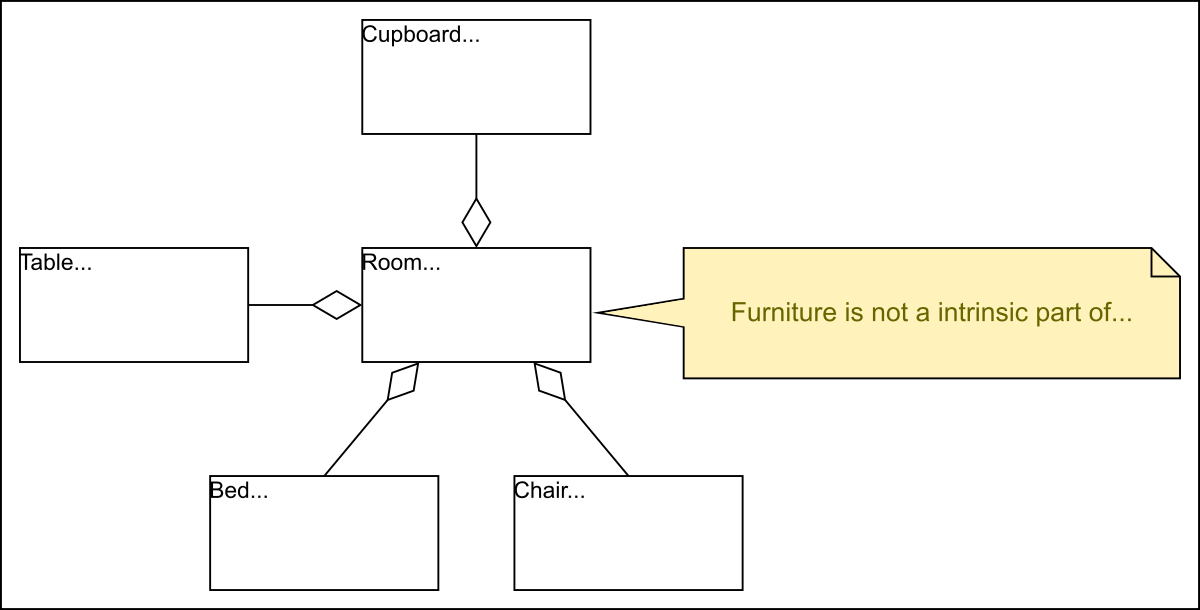
\includegraphics[width=0.5\textwidth]{Images/chapter_3/section_5678758717816832/4887024249339904.png}
 \caption{The class diagram of aggregation}
\end{figure}

\paragraph{Composition}\label{composition}
\\
An object may be composed of smaller objects, and the relationship between the ``part'' objects and ``whole'' objects is known as \textbf{composition}.
\\
In the example below, the \texttt{Chair} class can be composed of other objects of \texttt{Arm}, \texttt{Seat}, and \texttt{Leg} types. Composition is denoted by a line with a filled diamond head at the composer class pointing to the component class.
\\
Composition is a \emph{strong} relationship because:

\begin{itemize}
\item
The composed object becomes a part of the composer.
\item
Composed objects can not exist independently.
\end{itemize}

\begin{figure}[htbp]
 \centering
 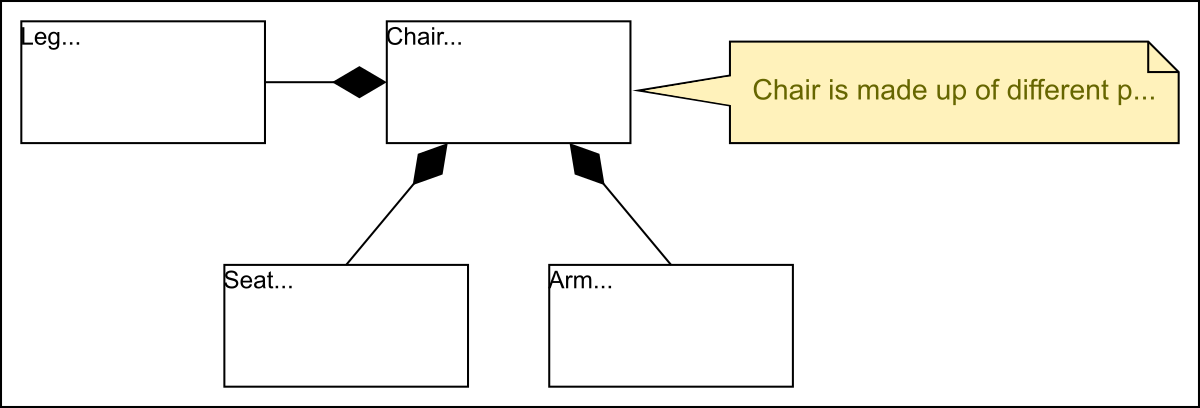
\includegraphics[width=0.5\textwidth]{Images/chapter_3/section_5678758717816832/6587968771063808.png}
 \caption{The class diagram of composition}
\end{figure}

\paragraph{Some additional types of association}\label{some-additional-types-of-association}
\\
The following are some types of simple associations based on navigation:

\begin{itemize}
\item
Single-direction navigation is called \textbf{one-way association} and is denoted by an arrow toward the server object.
\end{itemize}

\begin{figure}[htbp]
 \centering
 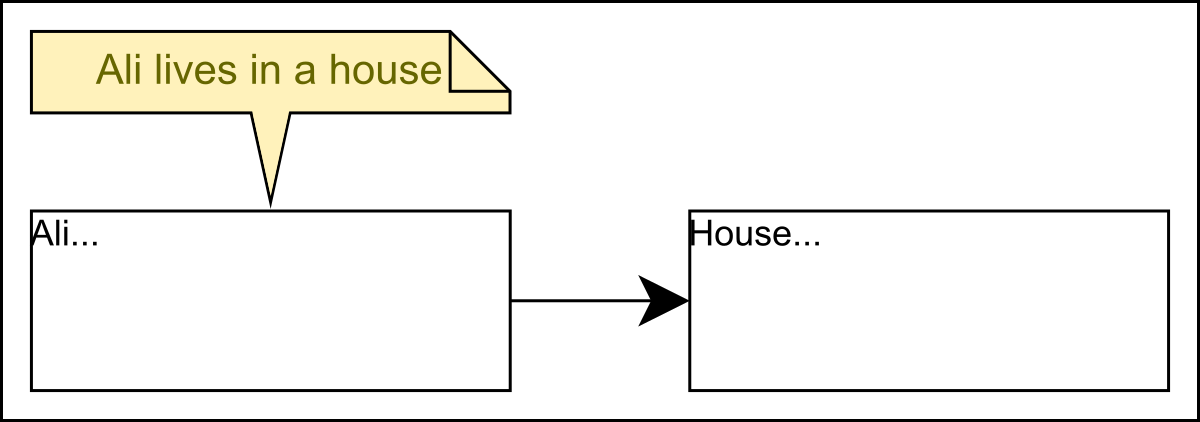
\includegraphics[width=0.5\textwidth]{Images/chapter_3/section_5678758717816832/6431631894380544.png}
 \caption{The class diagram of one-way association}
\end{figure}

\begin{itemize}
\item
If we navigate in both directions, the association is called a \textbf{two-way association} and is denoted by a line between two objects.
\end{itemize}

\begin{figure}[htbp]
 \centering
 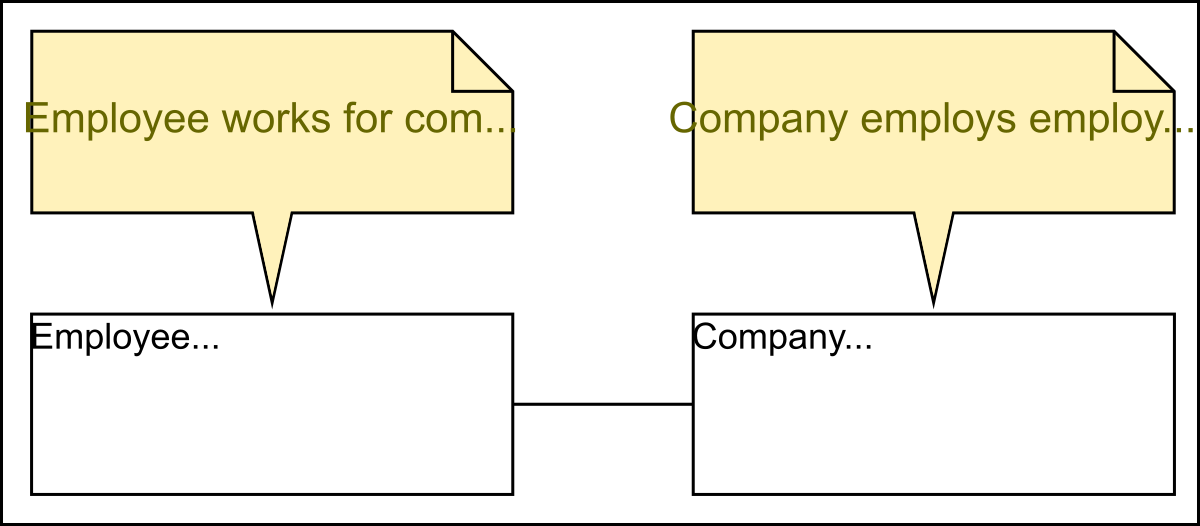
\includegraphics[width=0.5\textwidth]{Images/chapter_3/section_5678758717816832/5646870010658816.png}
 \caption{The class diagram of two-way association}
\end{figure}

\begin{itemize}
\item
Binary, ternary, and n-ary associations are based on the number of objects.

\begin{itemize}
\item
Association in which two objects are involved is called a \textbf{binary association.} The binary association includes one-way or two-way navigation.
\item
Association between the objects of exactly three classes is a \textbf{ternary association} and is denoted by a diamond with lines connected to associated objects.
\item
Association between more than three classes is called \textbf{n-ary} association.
\end{itemize}
\end{itemize}

\begin{figure}[htbp]
 \centering
 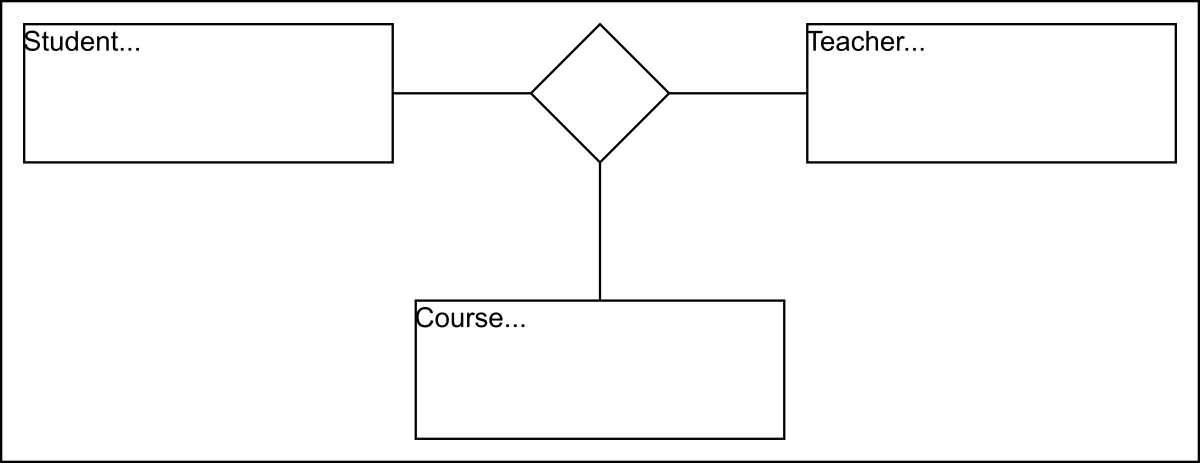
\includegraphics[width=0.5\textwidth]{Images/chapter_3/section_5678758717816832/5330996780335104.png}
 \caption{The class diagram of ternary association}
\end{figure}

\subsection{Dependency}\label{dependency}
\\
\textbf{Dependency} indicates that one class is dependent on another class(es) for its implementation. Another class may or may not depend on the first class. A dashed arrow denotes dependency.

\begin{figure}[htbp]
 \centering
 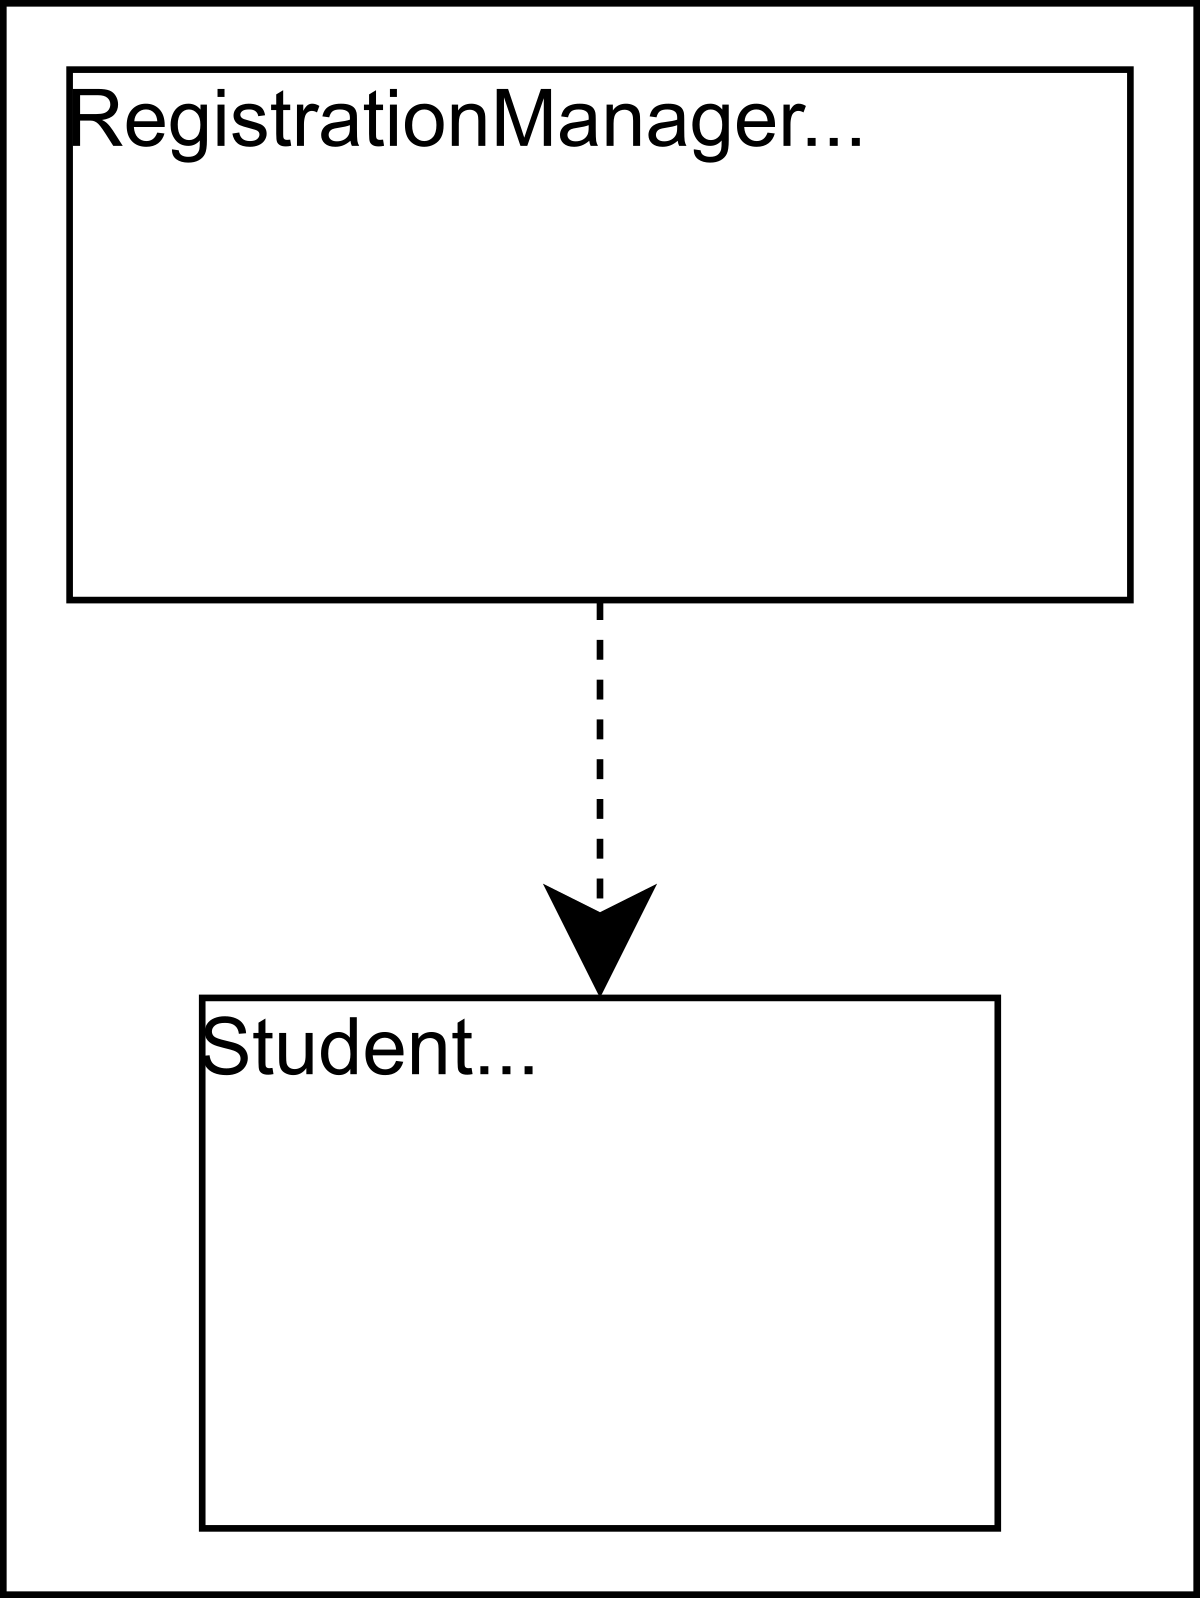
\includegraphics[width=0.25\textwidth]{Images/chapter_3/section_5678758717816832/6308492665421824.png}
 \caption{The class diagram representing dependency}
\end{figure}

In the example above, we have two classes---\texttt{RegistrationManager} and \texttt{Student}. The
\texttt{RegistrationManager} class relies on the \texttt{Student} class for its behavior because the object of the \texttt{Student} class is passed as a parameter to one of the functions in the \texttt{RegistrationManager} class.
\\
In the next lesson, we will look at the sequence diagram and its notation in detail.

% End of section content